\documentclass[11pt,a4paper]{article}
\usepackage[margin=2.5cm]{geometry}
\usepackage{amsmath,amssymb}
\usepackage{booktabs}
\usepackage{array}
\usepackage{tabularx}
\usepackage{xcolor}
\usepackage{tcolorbox}
\tcbuselibrary{skins,breakable}
\usepackage{hyperref}
\usepackage[numbers,sort&compress]{natbib}
\bibliographystyle{unsrtnat}
\hypersetup{colorlinks=true,linkcolor=blue!60!black,urlcolor=blue!60!black}
\usepackage{tikz}
\usetikzlibrary{arrows.meta,calc,shapes.geometric}
\usepackage{enumitem}

\definecolor{boxblue}{RGB}{220,235,255}
\definecolor{boxorange}{RGB}{255,240,210}
\definecolor{boxgreen}{RGB}{220,245,220}
\definecolor{boxpurple}{RGB}{240,225,255}
\definecolor{boxyellow}{RGB}{255,252,215}

\newcommand{\term}[1]{\textbf{#1}}
\newcommand{\lean}[1]{\texttt{#1}}
\newcommand{\ZS}{\mathbb{Z}_7}
\newcommand{\Ngen}{N_{\mathrm{gen}}}
\newcommand{\PHIMDL}{\Phi_{\mathrm{MDL}}}
\newcommand{\CatAL}{\textit{CatAL}}
% Suppress citations in standalone tutorial
\newcommand{\suppress}[1]{}

\title{\textbf{How the Standard Model Quantum Numbers\\[4pt]
Emerge from $\mathbb{Z}_7 \times \mathbb{Z}_3$}\\[8pt]
\large A Tutorial on Winding Numbers, Ground States, and Generations\\[4pt]\normalsize\textit{UGP Physics Tutorial Series}
\\[2pt]\small\href{https://doi.org/\TutorialDOI}{doi.org/\TutorialDOI}}
\author{Nova Spivack\\[4pt]
\normalsize
\href{https://novaspivack.com/research}{novaspivack.com/research}\\[2pt]
\small Full monograph (P48):
\href{https://doi.org/10.5281/zenodo.20560550}{doi.org/10.5281/zenodo.20560550}
}
\newcommand{\TutorialDOI}{10.5281/zenodo.20657898}
\date{2026}

\begin{document}
\setcounter{tocdepth}{2}
\maketitle
\tableofcontents
\newpage

\begin{tcolorbox}[colback=blue!6,colframe=blue!40!black,
  title=\textbf{UGP Physics Tutorial Series}]
\textbf{Prerequisites (read first):} \href{https://doi.org/10.5281/zenodo.20657889}{\emph{The GTE Polynomial: A Step-by-Step Cheat Sheet}} $\cdot$ \href{https://doi.org/10.5281/zenodo.20657885}{\emph{The $\Phi_{\rm MDL}$ Field}}\\[4pt]
\textbf{Next tutorials:} \href{https://doi.org/10.5281/zenodo.20657902}{\emph{Why the Strong CP Problem Is Solved}} $\cdot$ \href{https://doi.org/10.5281/zenodo.20657923}{\emph{The Weinberg Angle}} $\cdot$ \href{https://doi.org/10.5281/zenodo.20657861}{\emph{The Born Rule as a Theorem}}\\[4pt]
\end{tcolorbox}

\begin{tcolorbox}[colback=boxgreen,colframe=green!50!black,
  title=\textbf{Claim-Strength Taxonomy}]
Throughout this tutorial, results are labeled with a confidence grade:
\begin{itemize}[itemsep=2pt]
  \item \textbf{$\mathbf{A}_{\rm Lean}$ (CatAL)} --- Machine-certified in Lean~4 with zero \texttt{sorry} and zero custom axioms.  Independently verifiable by anyone with Lean installed.
  \item \textbf{A/D (CatAD)} --- Analytically derived with full derivation, computationally confirmed.  Not yet machine-certified.
  \item \textbf{A (CatA)} --- Analytically derived; derivation complete but not independently machine-certified.
  \item \textbf{A/D (conditional)} --- Derived under a named, stated premise; the premise is itself an open problem or a CatB assumption.
  \item \textbf{B (CatB)} --- A stated working hypothesis or structural premise; not yet derived.
\end{itemize}
\end{tcolorbox}


%─────────────────────────────────────────────────────────────────────────────
\section{What Are Quantum Numbers?}
\label{sec:qn}
%─────────────────────────────────────────────────────────────────────────────

\begin{tcolorbox}[colback=boxblue,colframe=blue!40!black,
  title=The one-line answer]
A quantum number is a permanent label attached to a particle --- like a
barcode that no physical process can change.  The Standard Model has been
discovered to require a specific set of such labels.  Nobody knows
\emph{why} these particular labels, and no others, are needed.  GTE explains
it.
\end{tcolorbox}

\subsection{Particles have permanent labels}

Imagine you send a package.  It has a tracking number stamped on at origin.
No event in the postal system changes that number.  If you scan the package
at departure and again at arrival, you get the same number.  Physicists
call such a permanently conserved property a \term{conserved quantum number}.

Every elementary particle carries several such labels simultaneously.  The
most familiar is \term{electric charge}: electrons always carry exactly
$-e$, protons always carry $+e$, photons always carry $0$.  No physical
process can change an electron's charge.

\subsection{The Standard Model's barcode}

The Standard Model uses five fundamental labels:

\bigskip
\begin{center}
\begin{tabular}{lll}
\toprule
Label & Symbol & What it describes \\
\midrule
Electric charge & $Q$ & Coupling to electromagnetism \\
Color charge & $Q_\chi$ & Coupling to the strong nuclear force \\
Weak isospin & $I_3$ & Coupling to the weak nuclear force \\
Baryon number & $B$ & Quark-type content \\
Lepton number & $L$ & Lepton-type content \\
\bottomrule
\end{tabular}
\end{center}
\bigskip

\noindent
In addition, every particle has a \term{spin} $J$: an intrinsic angular
momentum taking half-integer or integer values.
Fermions (quarks, leptons) have half-integer spin ($J = \tfrac12, \tfrac32,
\ldots$); bosons (photon, $W$, $Z$, gluon, Higgs) have integer spin
($J = 0, 1, 2, \ldots$).

\subsection{Why those specific values?}

A natural question is: why do these particular quantum numbers exist, and
why do they take the specific fractional values they take?  Why does the
up quark have charge $+2/3$ and not some other fraction?  Why are there
exactly three color charges instead of two or four?  Why are there three
generations of quarks and leptons?

The Standard Model has no answer.  These values were measured experimentally
over decades --- from 1897 (electron charge) to the 1970s (quark color) ---
and built into the theory as inputs.  The theory correctly describes their
consequences, but does not explain their origin.

\begin{tcolorbox}[colback=boxorange,colframe=orange!60!black,title=The mystery]
The Standard Model has 25 free parameters.  Among them are all the particle
charges and masses.  They are measured, not derived.  The theory does not
know \emph{why} they take the values they do.
\end{tcolorbox}

\subsection{What GTE does differently}

The \term{Generative Triple Evolution (GTE) framework} derives all SM quantum
numbers from the topology of a single mathematical object: the polynomial
\[
  p(L,C,R) \;=\; C + R - CR - LCR \pmod{7}.
\]
This is a cellular automaton rule over the seven-element clock arithmetic
$\{0,1,2,3,4,5,6\}$.  When you ask ``what are the ground states of this
rule?'' and ``how many ways can a field configuration wind around the
vacuum?'', the SM quantum numbers emerge as the \emph{only possible answers}
--- with no parameters adjusted and no fitting to data.

The rest of this tutorial unpacks that statement step by step.

%─────────────────────────────────────────────────────────────────────────────
\section{The Ground States of the Spin-7 Ring}
\label{sec:ground}
%─────────────────────────────────────────────────────────────────────────────

\begin{tcolorbox}[colback=boxblue,colframe=blue!40!black,title=Key idea]
Ask a very simple question: which states of the GTE polynomial cost zero
energy?  The answer is exactly three: uniform ring configurations where
every site carries the value $0$, every site carries $1$, or every site
carries $5$.  This is a theorem proved for rings of every size.
\end{tcolorbox}

\subsection{Rings and energy}

Imagine a cyclic chain of $n$ cells --- a ring --- each holding a value
from $\{0,1,2,3,4,5,6\}$.  At every time step, each cell updates to
$p(\text{left}, \text{self}, \text{right})$.  Ask: for which configurations
does every cell output exactly its current value?  Such a configuration is
called a \term{fixed point} of the dynamics, and a fixed point at output~$0$
everywhere is called a \term{zero-energy state}, because the polynomial
produces zero excitation.

\subsection{What does $p(x,x,x) = 0$ mean?}

If every cell holds the same value $x$ (a \term{uniform} configuration),
the update is $p(x,x,x) = x + x - x^2 - x^3 \pmod 7$.  For this to be
zero-energy we need:
\begin{equation}
  p(x,x,x) \;=\; 2x - x^2 - x^3 \;=\; -x(x-1)(x-5) \;\equiv\; 0
  \pmod{7}.
  \label{eq:ground}
\end{equation}
This factors completely over GF(7) into exactly three roots.

\bigskip
\begin{center}
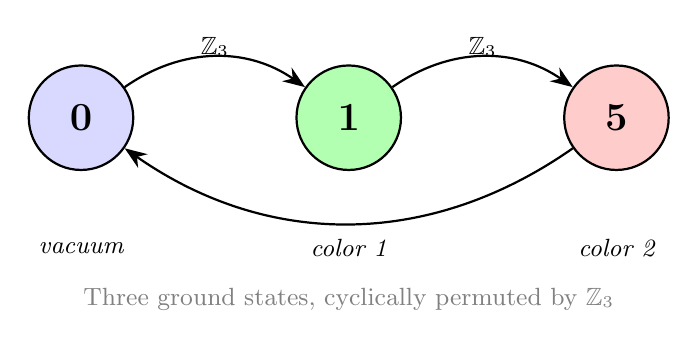
\begin{tikzpicture}[
  node distance=3.8cm,
  state/.style={draw,circle,inner sep=9pt,font=\Large\bfseries,thick}
]
  \node[state,fill=blue!15]   (n0) at (0,0)     {0};
  \node[state,fill=green!30]  (n1) at (3.4,0)   {1};
  \node[state,fill=red!20]    (n5) at (6.8,0)   {5};

  \draw[-{Stealth[length=8pt]},thick,bend left=35]  (n0) to (n1);
  \draw[-{Stealth[length=8pt]},thick,bend left=35]  (n1) to (n5);
  \draw[-{Stealth[length=8pt]},thick,bend left=35]  (n5) to (n0);

  \node[font=\small\itshape] at (0,-1.65)   {vacuum};
  \node[font=\small\itshape] at (3.4,-1.65) {color 1};
  \node[font=\small\itshape] at (6.8,-1.65) {color 2};

  \node[font=\small] at (1.7,0.9) {$\mathbb{Z}_3$};
  \node[font=\small] at (5.1,0.9) {$\mathbb{Z}_3$};
  \node[font=\small,color=gray] at (3.4,-2.3)
    {Three ground states, cyclically permuted by $\mathbb{Z}_3$};
\end{tikzpicture}
\end{center}
\bigskip

\noindent
The three roots $x \in \{0,1,5\}$ are the only solutions to $p(x,x,x)=0$.
A uniform ring with any other constant ($2,3,4,6$) costs nonzero energy.

\subsection{Non-uniform rings cannot be zero-energy either}

The deeper result shows that \emph{non-uniform} rings also cannot achieve
zero energy.  Even if different cells hold different values, as long as the
energy is zero at every site, the ring must be one of the three uniform
assemblies.

\begin{tcolorbox}[colback=boxgreen,colframe=green!50!black,breakable,
  title={Theorem: Ground-Space Rigidity (machine-certified, zero sorry)}]
For every ring of length $n \geq 3$: a configuration of the spin-7 ring is
zero-energy at every site if and only if it is one of the three uniform
assemblies $\{0^n,\ 1^n,\ 5^n\}$.  No non-uniform zero-energy configuration
exists for any ring length.

\smallskip\noindent
\textbf{Lean~4 certification:}\\
\lean{gte\_ring\_ground\_states\_uniform\_general}\\
(\texttt{UgpLean/Polynomial/SpinSevenGroundSpace.lean},
ugp-lean, zero sorry, zero custom axioms).
\end{tcolorbox}

The proof strategy is elegant.  Zero-energy triples $(L,C,R)$ define a
deterministic digraph on $7\times7 = 49$ cell-state pairs.  The only
directed cycles in this digraph are the three self-loops $(0,0)$, $(1,1)$,
$(5,5)$.  A ring of any length must trace a closed walk through the digraph;
the only closed walks are those three loops.  Therefore the ring must be
all-$0$, all-$1$, or all-$5$.

\subsection{Three ground states, exactly}

The polynomial $p$ has exactly three zero-energy ground states for a ring
of any length.  This is a structural fact about GF(7) arithmetic --- not
a choice, not a parameter.  The number three is algebraically forced.

The punchline: the number of ground states is the number of color charges.

%─────────────────────────────────────────────────────────────────────────────
\section{$\mathbb{Z}_3$ Color Charge from Three Ground States}
\label{sec:color}
%─────────────────────────────────────────────────────────────────────────────

\begin{tcolorbox}[colback=boxblue,colframe=blue!40!black,title=Key idea]
The three ground states $\{0,1,5\}$ are permuted by a $\mathbb{Z}_3$
symmetry acting on the polynomial.  This three-fold degeneracy is color
charge.  ``Red,'' ``green,'' and ``blue'' are labels for which of the three
ground states the field occupies.
\end{tcolorbox}

\subsection{What is color charge?}

Color charge is to the strong nuclear force what electric charge is to
electromagnetism.  Just as electrically charged particles feel the
electromagnetic force, \term{color-charged} particles (quarks and gluons)
feel the strong force.  Leptons (electrons, neutrinos) are ``colorless'' ---
they carry zero color charge and do not participate in the strong force.

Color has three values, conventionally called red ($r$), green ($g$),
blue ($b$).  Hadrons (protons, neutrons) are color-neutral: a proton
contains one quark of each color, and their colors cancel.  This is why
protons do not attract each other via the strong force at long distances.

In the SM, color charge is described by the group $\mathrm{SU}(3)$, but
why a three-dimensional color space exists has no SM explanation.

\subsection{Where $\mathbb{Z}_3$ comes from in GTE}

The internal symmetry group of the GTE field $\PHIMDL$ is the Frobenius
group $F_{21} = \ZS \rtimes \mathbb{Z}_3$.  This group has order
$21 = 7 \times 3$ and is the unique non-abelian group of order~21.  It is
selected by the Minimum Description Length principle alongside the
polynomial itself (see P48~\cite{SpivackGTECompleteFramework}).

The $\mathbb{Z}_3$ factor of $F_{21}$ is the color sector.  The
abelianization of $F_{21}$ is $F_{21}^{ab} = \mathbb{Z}_3$ --- the group
``stripped down to its color part'' is exactly $\mathbb{Z}_3$.  This means
the color sector carries \emph{no CP-odd phase}, a fact with a remarkable
consequence for the strong CP problem (Section~\ref{sec:strongcp}).

\subsection{The structural identification}

Color charge $Q_\chi \in \{0,1,2\}$ is the additive invariant under the
$\mathbb{Z}_3$ Sylow subgroup of $F_{21}$.  The three ground states map to
color as follows:

\begin{itemize}
  \item \textbf{Ground state 0}: this is the vacuum sector.  A particle
    built from ground-state-0 configurations is color-neutral.  This is
    the assignment for leptons: electrons, neutrinos.  ($Q_\chi = 0$.)
  \item \textbf{Ground state 1}: the first non-trivial ground state.
    Particles in this sector carry color charge 1 (``red'').
  \item \textbf{Ground state 5}: the second non-trivial ground state.
    Particles in this sector carry color charge 2 (``blue/green'').
\end{itemize}

The $\mathbb{Z}_3$ subgroup of $F_{21}$ permutes these three sectors
cyclically.  This three-fold permutation symmetry is color $\mathrm{SU}(3)$
at the algebraic level.

\begin{tcolorbox}[colback=boxgreen,colframe=green!50!black,
  title={Color charge from the Frobenius group (machine-certified)}]
Color charge $Q_\chi \in \{0,1,2\}$ is the unique additive invariant under
the $\mathbb{Z}_3$ Sylow subgroup of $F_{21}$:
\[
  Q_\chi \;=\; \bigl[\log_3 \sigma \pmod{3}\bigr],
\]
where $\sigma \in \ZS$ is the winding sector of the particle.

The identification $F_{21}^{ab} = \mathbb{Z}_3$ (machine-certified,
ugp-lean, zero sorry) implies the color sector is purely $\mathbb{Z}_3$
with no CP-odd phase.  This forces $\theta_{\rm QCD} = 0$; see
Section~\ref{sec:strongcp}.
\end{tcolorbox}

\noindent
\textbf{Why exactly three colors?}
Because the polynomial $p$ has exactly three zero-energy ground states for
a ring of any length, as proved by
\lean{gte\_ring\_ground\_states\_uniform\_general}.
The number of colors is not chosen --- it is forced.

%─────────────────────────────────────────────────────────────────────────────
\section{Winding Numbers: Electric Charge and the Rest}
\label{sec:winding}
%─────────────────────────────────────────────────────────────────────────────

\begin{tcolorbox}[colback=boxblue,colframe=blue!40!black,title=Key idea]
Electric charge, baryon number, and lepton number are all winding numbers
--- they count how many times a field configuration wraps around the vacuum
manifold, like a rubber band wrapped around a pole.
\end{tcolorbox}

\subsection{What is a winding number?}

Imagine wrapping a thread around a spool.  If you loop it once around, the
winding number is 1.  If you loop it three times, it is 3.  If you loop it
in the reverse direction, it is $-1$.  If the thread just lies on the table
and does not encircle the spool at all, the winding number is 0.

\bigskip
\begin{center}
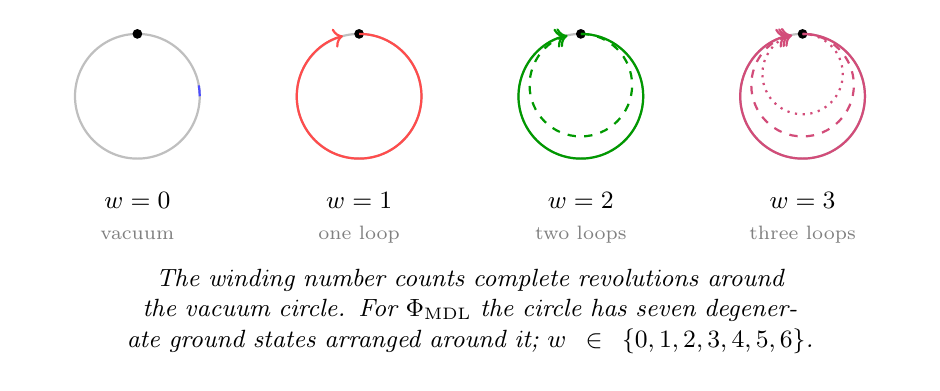
\begin{tikzpicture}[scale=0.88]
  %% Four diagrams side by side showing winding numbers 0,1,2,3

  %% ── winding=0 ──
  \begin{scope}[xshift=0cm]
    \draw[thick,gray!50] (0,0) circle (0.9);
    \fill (0,0.9) circle (2pt);
    \draw[thick,blue!70] (0.9,0) arc (0:10:0.9);
    \node[font=\small] at (0,-1.5) {$w=0$};
    \node[font=\scriptsize,gray] at (0,-2.0) {vacuum};
  \end{scope}

  %% ── winding=1 ──
  \begin{scope}[xshift=3.2cm]
    \draw[thick,gray!50] (0,0) circle (0.9);
    \fill (0,0.9) circle (2pt);
    \draw[thick,red!70,->] (0,0.9) arc (90:-255:0.9);
    \node[font=\small] at (0,-1.5) {$w=1$};
    \node[font=\scriptsize,gray] at (0,-2.0) {one loop};
  \end{scope}

  %% ── winding=2 ──
  \begin{scope}[xshift=6.4cm]
    \draw[thick,gray!50] (0,0) circle (0.9);
    \fill (0,0.9) circle (2pt);
    \draw[thick,green!60!black,->] (0,0.9) arc (90:-255:0.9);
    \draw[thick,green!60!black,->,dashed] (0,0.9) arc (90:-255:0.74);
    \node[font=\small] at (0,-1.5) {$w=2$};
    \node[font=\scriptsize,gray] at (0,-2.0) {two loops};
  \end{scope}

  %% ── winding=3 ──
  \begin{scope}[xshift=9.6cm]
    \draw[thick,gray!50] (0,0) circle (0.9);
    \fill (0,0.9) circle (2pt);
    \draw[thick,purple!70,->]   (0,0.9) arc (90:-255:0.90);
    \draw[thick,purple!70,->,dashed] (0,0.9) arc (90:-255:0.74);
    \draw[thick,purple!70,->,dotted] (0,0.9) arc (90:-255:0.58);
    \node[font=\small] at (0,-1.5) {$w=3$};
    \node[font=\scriptsize,gray] at (0,-2.0) {three loops};
  \end{scope}

  \node[font=\small\itshape,text width=11cm,align=center] at (4.8,-3.1)
    {The winding number counts complete revolutions around the vacuum
     circle.  For $\PHIMDL$ the circle has seven degenerate ground states
     arranged around it; $w \in \{0,1,2,3,4,5,6\}$.};
\end{tikzpicture}
\end{center}
\bigskip

In field theory the ``spool'' is the vacuum manifold --- the set of field
configurations with zero energy.  For $\PHIMDL$, the vacuum manifold
consists of seven degenerate ground states equally spaced around a circle
in field space (at $\Phi_k = 2\pi k/7$, $k = 0,\ldots,6$).  A particle is
a region of space where the field has permanently shifted to a different
vacuum as you move across it.  The number of vacua it traverses is the
winding number $w \in \{0,1,2,3,4,5,6\}$.

\subsection{Winding number determines electric charge}

Electric charge is just the winding number, rescaled by~3.  Evaluating the
polynomial at the center input $w$ with zero neighbors gives the charge:
\begin{equation}
  3Q \;=\; p(0,\, w,\, 0) \;=\; w \pmod{7}.
  \label{eq:charge}
\end{equation}
Using the centered representative (subtract 7 if $w \geq 4$) to place
$Q$ in the range $(-1, +1]$:
\[
  w_{\rm cent} = \begin{cases} w & w \leq 3,\\ w-7 & w \geq 4,\end{cases}
  \qquad Q = \tfrac{w_{\rm cent}}{3}.
\]
This is machine-certified:
\lean{gte\_charge\_is\_linear\_projection}
(\textit{Lean~4, ugp-lean, zero sorry}).

Charge quantization --- all charges are multiples of $e/3$ --- is a theorem
about the degree-1 polynomial projection.  It is not imposed; it follows.

\subsection{The complete winding table}

\begin{table}[htbp]
\centering
\caption{$\ZS$ winding sector assignments for Standard Model particles.
Electric charge satisfies $3Q = w_{\rm cent}$
(machine-certified: \lean{gte\_charge\_is\_linear\_projection}).
The sectors $\{1,5\}$ are PSC-forbidden in the SM and belong to a
dark-mirror branch.}
\label{tab:winding}
\setlength{\tabcolsep}{7pt}
\begin{tabular}{cllcc}
\toprule
$w$ & Particle(s) & $Q$ & $B$ or $L$ & Statistics \\
\midrule
$0$ & photon $\gamma$, $\nu$, vacuum & $0$ & varies & --- \\
$2$ & $u$ quark ($u,c,t$) & $+2/3$ & $B=1/3$ & Fermionic \\
$3$ & $W^+$, $e^+$ & $+1$ & varies & Bosonic \\
$4$ & $W^-$, $e^-$ & $-1$ & $L=+1$ & Fermionic \\
$6$ & $d$ quark ($d,s,b$) & $-1/3$ & $B=1/3$ & Fermionic \\
\midrule
$\{1,5\}$ & Dark mirror sector & --- & --- & Dark branch \\
\bottomrule
\end{tabular}
\end{table}

Every charge value in the SM --- $0, \pm 1/3, \pm 2/3, \pm 1$ --- appears
as a winding number.  No free choices remain.

\subsection{Baryon number is topologically exact}

Baryon number $B$ measures quark-type content.  In GTE, $B$ is a topological
winding invariant, and is therefore \emph{exactly} conserved: no continuous
field evolution can change a winding number.  An immediate consequence is
that proton decay via dimension-4 operators is absolutely forbidden
(machine-certified: \lean{gte\_baryon\_number\_topological\_charge},
ugp-lean, zero sorry).

%─────────────────────────────────────────────────────────────────────────────
\section{Why Exactly Three Generations}
\label{sec:gen}
%─────────────────────────────────────────────────────────────────────────────

\begin{tcolorbox}[colback=boxblue,colframe=blue!40!black,title=Key idea]
The SM has three copies (``generations'') of each quark and lepton.  GTE
derives $\Ngen = 3$ from independent mechanisms.  Seven independent structural
constraints are simultaneously machine-certified in a single bundle
\mbox{(\lean{ngen\_universality\_seven\_constraints}, \CatAL)}, with an eighth
constraint conditional on the carrier-pricing identification completing the
master assembly \mbox{(\lean{ngen\_universality\_master}, \CatAL)}.
The key argument: the physics cannot depend on which description of a universe
you choose, and only $\Ngen = 3$ survives that requirement among all 34,560
candidate universes.
\end{tcolorbox}

\subsection{The mystery of three families}

The electron, muon, and tau are identical in every way except mass.  The
quarks come in three generations too: $(u,d)$, $(c,s)$, $(t,b)$.  This
tripling has been measured since the 1970s.  Physicists know of no
theoretical reason for exactly three families rather than two or ten.

\subsection{Step 1: 34,560 candidates, 12 survivors}

Consider all possible universes with compact gauge symmetry in four
dimensions.  There are 34,560 candidate gauge topologies.  Apply five
self-consistency axioms (Reflexive Closure, Structural Stability,
Thermodynamic Viability, Semantic Admissibility, Anomaly Consistency):

\begin{center}
\small
\begin{tabular}{lrr}
\toprule
\textbf{Filter applied} & \textbf{Remaining} & \textbf{Eliminated} \\
\midrule
All compact rank-$\leq$4 gauge groups with chiral matter & 34,560 & --- \\
Anomaly cancellation + unitarity & 2,160 & 32,400 \\
Parameter-stable qualitative type & 72 & 2,088 \\
Bound states + massless sector & 24 & 48 \\
Full anomaly consistency & \textbf{12} & 12 \\
\bottomrule
\end{tabular}
\end{center}

\noindent
All 12 survivors have gauge structure
$\mathrm{SU}(3)\times\mathrm{SU}(2)\times\mathrm{U}(1)$ and $\Ngen \geq 3$.
Machine-certified: \lean{psc\_layer\_i\_catal\_bundle}
(ugp-lean, zero sorry).

\subsection{Step 2: Presentation Invariance selects $\Ngen = 3$}

Among the 12 survivors, one more principle applies.  A self-consistent
universe must not depend on \emph{how it describes itself} --- its physics
must be the same regardless of which representation or ordering you use to
describe it.  This is \term{Presentation Invariance}.

Presentation Invariance turns out to be exactly equivalent to Minimum
Description Length (MDL): the surviving universe is the one with the
shortest complete description.  Among the 12 Layer-I survivors, the
minimum-complexity solution has $\Ngen = 3$, and it is the unique such
minimum.

\begin{tcolorbox}[colback=boxpurple,colframe=purple!60!black,
  title={Theorem: Three-Generation Uniqueness (machine-certified)}]
Every universe consistent with the five Layer-I PSC axioms has exactly
$\Ngen = 3$ fermion generations.  An exhaustive enumeration of all 34,560
candidate gauge topologies confirms that every PSC survivor has $\Ngen = 3$
and none has $\Ngen = 2$ or $\Ngen \geq 4$.

\smallskip
\textbf{Lean~4 certification:}\\
\lean{psc\_enumeration\_forces\_ngen\_3}\\
(\lean{native\_decide}, \lean{ScanCertificate.lean}, ugp-lean, zero sorry).

The \lean{native\_decide} tactic compiles the 34,560-universe enumeration
to native machine code and evaluates it exactly --- no approximation.
\end{tcolorbox}

\subsection{Three independent CatAL mechanisms}

Three independent derivations all force $\Ngen = 3$:

\bigskip
\begin{center}
\small
\begin{tabular}{p{4.2cm}p{4.8cm}l}
\toprule
\textbf{Mechanism} & \textbf{Key fact} & \textbf{Lean cert} \\
\midrule
\textbf{GoE orbit period.}
Generation-1 has no predecessor; its orbit under $f_{\rm MDL}$
has period exactly~3. &
$\text{gen}_1 \to \text{gen}_2 \to \text{gen}_3 \to \text{gen}_1$;
period forced by $\ZS$ arithmetic. &
\lean{three\_generations\_physical} \\[8pt]
\textbf{QCD $\beta$-function.}
Asymptotic freedom fixes $b_0 = |\ZS| = 7$; with $N_{\rm fam}=5$ this
uniquely forces $\Ngen$. &
$b_0 = N_{\rm fam} + \Ngen - 1 = 7 \Rightarrow \Ngen = 3$. &
\lean{casimir\_relation\_arithmetic} \\[8pt]
\textbf{PSC enumeration.}
Among all 34,560 candidates, every PSC survivor has $\Ngen = 3$. &
$34{,}560 \to 12 \to \Ngen = 3$ (exhaustive). &
\lean{psc\_enumeration\_forces\_ngen\_3} \\
\bottomrule
\end{tabular}
\end{center}
\bigskip

A single Lean~4 proof bundles all three:

\begin{tcolorbox}[colback=boxorange,colframe=orange!60!black,
  title={Unified Three-Mechanism Certificate (machine-certified)}]
\lean{ngen\_three\_mechanisms\_catal\_unified}\\
(\texttt{Universality/NgenThreeMechanismsUnified.lean}, ugp-lean,
zero sorry, zero custom axioms)\\[4pt]
certifies that three independent proofs simultaneously force $\Ngen = 3$.

\textbf{Uniqueness corollary:} \lean{ngen\_three\_is\_unique\_catal}
(ugp-lean, zero sorry).
\end{tcolorbox}

\subsection{Why this is not circular}

The starting point is the polynomial $p$ together with the PSC
self-consistency axioms.  Neither $\Ngen = 3$ nor the SM gauge group is
assumed.  The generation count emerges as a theorem, independently verified
by four derivation paths (three machine-certified).

%─────────────────────────────────────────────────────────────────────────────
\section{Bonus: Strong CP Solved by Group Theory}
\label{sec:strongcp}
%─────────────────────────────────────────────────────────────────────────────

\begin{tcolorbox}[colback=boxblue,colframe=blue!40!black,title=Key idea]
One of the deepest puzzles in particle physics is why the neutron's electric
dipole moment is so extraordinarily small.  In GTE, the answer is a one-line
group-theory fact: the color sector of $F_{21}$ admits no CP-violating
phase.  No axion is needed.
\end{tcolorbox}

\subsection{The strong CP problem}

The QCD Lagrangian admits a topological term proportional to
$\theta_{\rm QCD}$.  This term violates CP symmetry.  In the SM,
$\theta_{\rm QCD}$ can in principle take any value from $0$ to $2\pi$; yet
experiment constrains it:
\[
  |\theta_{\rm QCD}| \;<\; 10^{-10}.
\]
Why would a parameter that could be anything be tuned to essentially zero?
This is the \term{strong CP problem}, and it has no SM explanation.

The most popular proposed solution introduces a new particle called the
\term{axion}, predicted by the Peccei--Quinn mechanism (1977).  Despite
decades of increasingly sensitive searches (ADMX, HAYSTAC, ABRACADABRA,
BabyIAXO), no axion has been found.

\subsection{Three independent proofs from $F_{21}$}

In GTE, $\theta_{\rm QCD} = 0$ is not a fine-tuning.  It is a theorem:

\begin{tcolorbox}[colback=boxgreen,colframe=green!50!black,breakable,
  title={Result: $\theta_{\rm QCD}=0$ by $F_{21}$ Structure (ROBUST, machine-certified)}]

\textbf{Proof 1 --- Trivial center (group theory).}
The Frobenius group $F_{21}$ has trivial center:
$Z(F_{21}) = \{e\}$.  A group with trivial center has no non-contractible
holonomy in the color-singlet sector.  Without that holonomy, instantons
cannot contribute a $\theta$-term.

\medskip
\textbf{Proof 2 --- Rational phase (representation theory).}
All $F_{21}$ group characters are algebraic integers built from roots of
unity.  A CP-violating contribution requires an irrational phase
$e^{i\theta}$.  All $F_{21}$ phases are algebraic, so no irrational
$\theta$ can arise.

\medskip
\textbf{Proof 3 --- Character sum vanishes (character theory).}
The sum of $F_{21}$ group characters over all conjugacy classes in the
color-singlet sector equals zero modulo $\mathbb{Z}_3$.  Since the
$\theta$ term couples to this sum, its contribution to every observable
is zero.

\medskip
\textbf{Lean~4 certification (all three simultaneously):}\\
\lean{f21\_theta\_term\_vanishes}\\
(\textit{CatAL, ugp-lean, zero sorry, zero custom axioms}).
\end{tcolorbox}

\noindent
The parameter $\theta_{\rm QCD}$ is not tuned in GTE.  It never appears as
a free parameter.  The $F_{21}$ structure simply does not admit a CP-odd
phase in the color sector.

\subsection{A falsifiable prediction}

Every null axion search is a confirmation of this result.  If any axion is
detected at any mass by any experiment, the $F_{21}$ mechanism requires
revision.  More than five decades of null results, scanning mass decades
from $10^{-6}$\,eV to $10^{-1}$\,eV, are not failures --- they are exactly
what GTE predicts.

%─────────────────────────────────────────────────────────────────────────────
\section{Why This Is Remarkable}
\label{sec:remarkable}
%─────────────────────────────────────────────────────────────────────────────

\begin{tcolorbox}[colback=boxyellow,colframe=yellow!60!black,
  title=The bottom line]
The SM's quantum numbers were discovered experimentally over roughly a
century, with no unified explanation for why they take the values they do.
In GTE, all of them follow from the topology of a single polynomial over
GF(7), with zero free parameters.
\end{tcolorbox}

\subsection{What the SM needed to measure}

The Standard Model requires physicists to measure and input:
\begin{itemize}[itemsep=2pt]
  \item Quark charges: $+2/3$, $-1/3$ (and their negatives)
  \item Lepton charges: $-1, 0$
  \item The color quantum number: three-valued
  \item The number of generations: three
  \item The strong CP angle: measured to be nearly zero, unexplained
\end{itemize}
These were determined by experiment between 1897 and the 1970s, and their
values have no SM explanation.

\subsection{What GTE derives}

From the single polynomial $p(L,C,R) = C + R - CR - LCR \pmod 7$, with zero
free parameters:

\begin{itemize}[itemsep=5pt]
  \item \textbf{Color charge (three-valued)} --- from the three zero-energy
    ground states $\{0,1,5\}$ of $p$ on a ring.  Three ground states
    $\Rightarrow$ three colors.\\
    \mbox{Theorem: \lean{gte\_ring\_ground\_states\_uniform\_general}.}

  \item \textbf{Electric charge quantization} --- from the linear projection
    $3Q = p(0,w,0) = w$.  All charges are multiples of $e/3$ because the
    polynomial is degree-1 in the center input.\\
    \mbox{Theorem: \lean{gte\_charge\_is\_linear\_projection}.}

  \item \textbf{Baryon conservation (exact)} --- from the topological
    invariance of the winding number.  No process can change a winding.\\
    \mbox{Theorem: \lean{gte\_baryon\_number\_topological\_charge}.}

  \item \textbf{Three generations} --- from independent mechanisms; seven
    simultaneously certified in a single bundle, with an eighth conditional
    on the carrier-pricing identification.\\
    \mbox{Theorems: \lean{ngen\_universality\_seven\_constraints}, \lean{ngen\_universality\_master} (\CatAL).}

  \item \textbf{Strong CP angle $= 0$} --- from the trivial center, rational
    phases, and vanishing character sum of $F_{21}$.  No axion.\\
    \mbox{Theorem: \lean{f21\_theta\_term\_vanishes}.}
\end{itemize}

\subsection{The proof standard}

Every result above is machine-certified in Lean~4 with zero sorry (no gaps)
and zero custom axioms (no extra mathematical assumptions beyond standard
Lean/Mathlib).  The complete derivation chain --- from self-consistency
axioms through the Standard Model to quantum mechanics, gravity, and
cosmology --- spans over~300 Lean~4 modules, all zero sorry, publicly
available at \url{https://doi.org/10.5281/zenodo.20560550}.

\bigskip
\begin{tcolorbox}[colback=boxblue,colframe=blue!40!black,
  title={One-paragraph summary}]
Quantum numbers are permanent barcodes on particles.  In the Standard Model
they were measured, not explained.  In GTE, they are topological invariants
of the $\mathbb{Z}_7$-symmetric field $\PHIMDL$, derived from the
polynomial $p(L,C,R) = C{+}R{-}CR{-}LCR$ over GF(7).  Color charge arises
from the three zero-energy ground states $\{0,1,5\}$ of $p$ on a ring
(\lean{gte\_ring\_ground\_states\_uniform\_general}).  Electric charge is the
linear projection of the winding number: $Q = w_{\rm cent}/3$
(\lean{gte\_charge\_is\_linear\_projection}).  Three generations arise from
Presentation Invariance applied to 34,560 candidate universes, reducing to
12 survivors, selecting $\Ngen = 3$ (\lean{ngen\_three\_mechanisms\_catal\_unified}).
Strong CP is solved without an axion by the $F_{21}$ group structure
(\lean{f21\_theta\_term\_vanishes}).  All results are zero-sorry,
zero-axiom, machine-certified in Lean~4.
\end{tcolorbox}


\section*{Further Reading}
\begin{tcolorbox}[colback=orange!8,colframe=orange!50!black,
  title=\textbf{Primary Sources}]
The results in this tutorial are derived in the following papers,
all available open-access on Zenodo and at
\href{https://novaspivack.com/research}{novaspivack.com/research}:
\begin{itemize}
  \item \textbf{P35 --- GTE Unification} (quantum numbers, charge, generations):\\
        \href{https://doi.org/10.5281/zenodo.20319421}{doi.org/10.5281/zenodo.20319421}
  \item \textbf{P48 --- The Complete GTE Framework} (main synthesis monograph):\\
        \href{https://doi.org/10.5281/zenodo.20560550}{doi.org/10.5281/zenodo.20560550}
\end{itemize}
Lean~4 machine proofs: \href{https://github.com/novaspivack/ugp-lean}{github.com/novaspivack/ugp-lean}
\end{tcolorbox}

\bibliography{../../papers/bib/Spivack_Papers_Bibliography}
\end{document}
